\documentclass[aps,prd,twocolumn,superscriptaddress,nofootinbib,amsmath,amssymb]{revtex4-2}
\usepackage{graphicx}
\usepackage{hyperref}
\usepackage{color}
\usepackage{bm}

\begin{document}
\title{\textbf{ANALYSIS AND OPTIMIZATION ON PIPE CRACK DETECTION WITH GAMMA COMPTON BACKSCATTERING USING TOMOGRAPHY AND GEANT4}}

% ==============================================================================
% AUTHOR LIST (Inlined from COSINE-100_authors_March2026_v3.tex)
% ==============================================================================
\author{\textbf{A.~N.~Rohman}}
\email{ardiansah.nur.2303226@students.um.ac.id}
\affiliation{Department of Physics, Universitas Negeri Malang, Malang 65145, Indonesia}
\author{\textbf{H.~Prihtiadi}}
\email{hafizh.fmipa@um.ac.id}
\affiliation{Department of Physics, Universitas Negeri Malang, Malang 65145, Indonesia}
%\collaboration{COSINE-100 Collaboration}\noaffiliation
% ==============================================================================

\begin{abstract}
Lorem ipsum dolor sit amet.
\end{abstract}

\maketitle

\section{Introduction}
Oil and gas pipe frequently exposed by corosif environment, i.e sour gas that contains Hydrogen Sulfide (H2S)\cite{Parishan2026}. This toxic compound can do the chemical reaction with the pipe fast enough to damage the pipe material, especially on the wielding joint and on the local stress point\cite{Parishan2026}. Then phenomena such Flow Acceleration Corrosion (FAC) cause the metal pipe wall erode and thin from the inside\cite{Elhoushy2018}.Failure to detect wall thinning or cracks at the earliest possible stage can lead to pipe rupture, leaks, environmental damage, risks to human, and massive financial losses due to operational shutdowns\cite{Wong2021}.  

Non-Destructive Testing/NDT are the inspection process, testing, and evaluation used to inspecting and analyzing material characteristic, component, or the structure without damaging the piping system itself\cite{Sari2019,Tai2025}. On piping aplication, NDT used to reach the area above ground that cannot being detected by visual, to detect the defects such as pipe wall thinning(metal loss), corossion, cracks, blockages, voids, or damages to welded joints\cite{Li2024}. Some commonly used NDT methods for pipelines include Ultrasonic Testing (UT), Radiography (RT), Acoustic Emission Testing, Magnetic Flux Leakage (MFL), and X-ray or gamma-ray backscattering techniques \cite{Sari2017}.

Conventional NDT like Ultrasonic Testing (UT), Radiographic Transmission, or Magnetic Flux Leakage (MFL) have some limitation, especially when applied on thick industrial pipe, buried underground pipe, and coated pipe with insulation. Highly recommended using Gamma Compton Backscatter because this technique offer revolutionary advantage to offset weakness of traditional NDT \cite{Elhoushy2018}. Traditional NDT require two side of the pipe simultaneously, namely radiation source and the detector in other side. This methode is way more difficult or even impossible if the pipe buried underground or have thick wall\cite{Sari2019}. Gamma Compton Backsacttering NDT solve this problem with placing the detector on the same side with the radiation source, this methode is ideal and practical for underground pipe or massive object\cite{Elhoushy2018}.

Compton scattering technique with Cs-137 have a good sensitivity for detecting depletion of the pipe, but the sensitivity is drop when the thickness of pipe more than 10 mm to 2,5 cm\cite{Elhoushy2018}. Most of all the instrument of gamma scattering stil operate with scanning the object point by point, it takes so many time and the scanning area is limited (i.e diamater 2 cm).

\section{METHOD AND SIMULATION}

\begin{figure}[htbp]
  \centering
  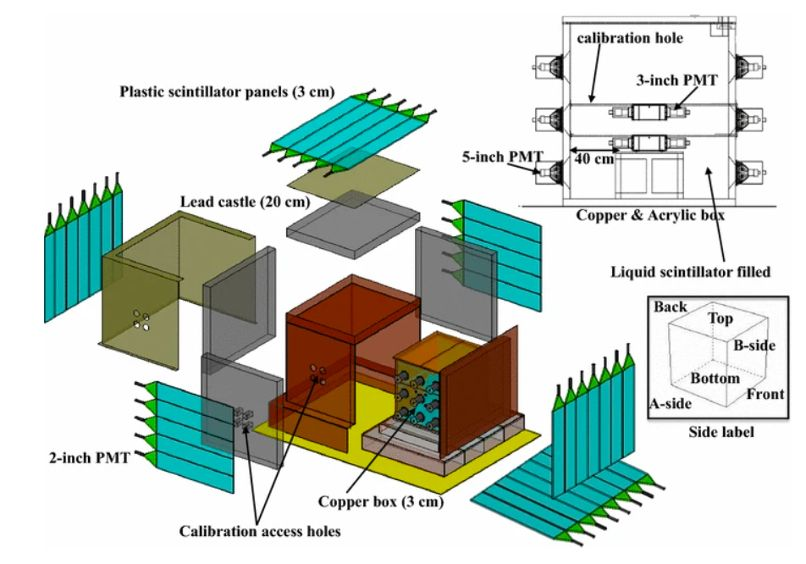
\includegraphics[width=\linewidth]{cosine_structure.jpeg}
  \caption{Schematic of the COSINE-100 detector. The NaI(Tl) crystals are immersed in the 2,200\,L LAB-LS and surrounded by layers of copper and lead shielding.}
  \label{fig:detector}
\end{figure}

\subsection{Relocation to Yemilab}


\subsection{Direct PMT-Coupling Architecture}

\begin{figure}[htbp]
  \centering
  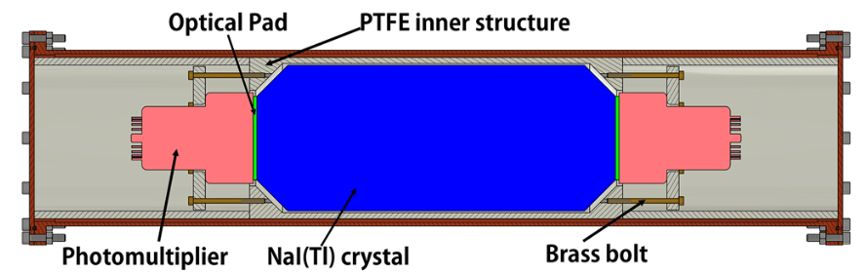
\includegraphics[width=\linewidth]{encapsulation_design_cosineu.jpeg}
  \caption{Cross-sectional view of the new NaI(Tl) crystal encapsulation for the COSINE-100U phase, illustrating the direct PMT-coupling without a quartz window.}
  \label{fig:encapsulation}
\end{figure}

\subsection{Liquid Scintillator Veto}

\begin{figure}[htbp]
  \centering
  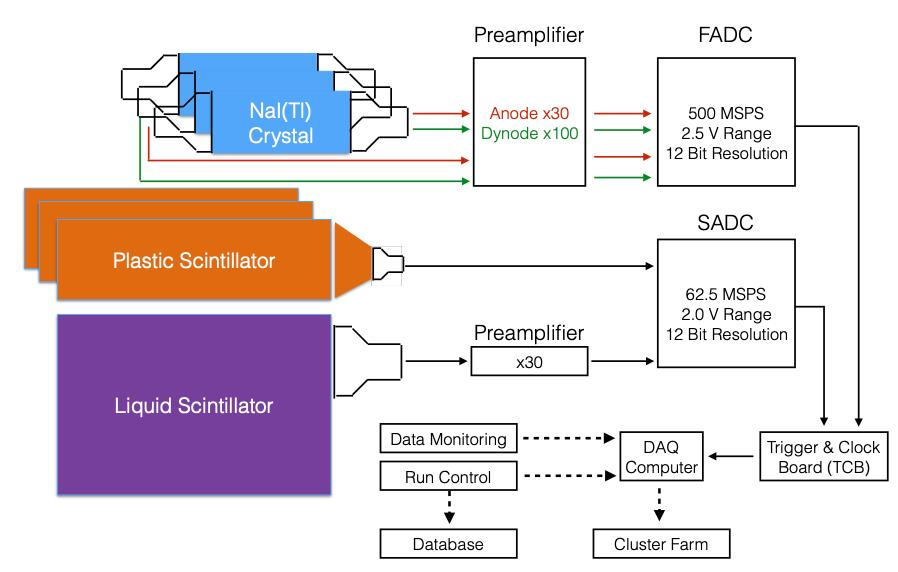
\includegraphics[width=\linewidth]{block_diagram_cosine.jpeg}
  \caption{Block diagram of the data acquisition (DAQ) and signal routing for the COSINE-100 experiment.}
  \label{fig:daq}
\end{figure}


\begin{equation}
    \ln\mathcal{L}(\bm{\theta}) = \sum_i \left( n_i \ln \nu_i(\bm{\theta}) - \nu_i(\bm{\theta}) \right),
\end{equation}
w
\section{RESULTS AND DISCUSSION}


\begin{figure}[htbp]
  \centering
  \framebox{\parbox{0.4\textwidth}{\centering
    \vspace{3cm}
    \textbf{[input gambar spectrum fit].pdf}
    \vspace{3cm}
  }}
  \caption{Projected energy spectrum of the COSINE-100U detectors from 0 to 20\,keVee of best-fit background model comprising $^{40}\mathrm{K}$, $^{210}\mathrm{Pb}$, and other intrinsic components.}
  \label{fig:expected_bg}
\end{figure}



\begin{table*}[htbp]
\centering
\caption{Single-hit event rates for major background sources and data in the 0.7 to 6 keV range, with error values representing the $1\sigma$ likelihood fit uncertainty.}
\label{tab:background_rates}
\begin{tabular}{l c c c c c}
\hline\hline
Unit [Counts/kg/keV/day] & Crystal 2 & Crystal 3 & Crystal 4 & Crystal 6 & Crystal 7 \\
\hline
Data & $-$ & $-$ & $-$ & $-$ & $-$ \\
Total simulation & $-$ & $-$ & $-$ & $-$ & $-$ \\
\hline
\textbf{Internal} & & & & & \\
\quad $^{210}$Pb & $-$ & $-$ & $-$ & $-$ & $-$ \\
\quad $^{40}$K & $-$ & $-$ & $-$ & $-$ & $-$ \\
\quad Others & $-$ & $-$ & $-$ & $-$ & $-$ \\
\hline
\textbf{Surface} & & & & & \\
\quad Crystal surface $^{210}$Pb & $-$ & $-$ & $-$ & $-$ & $-$ \\
\quad PTFE $^{210}$Pb & $-$ & $-$ & $-$ & $-$ & $-$ \\
\quad Copper K-shell X-ray & $-$ & $-$ & $-$ & $-$ & $-$ \\
\hline
\textbf{Cosmogenics} & & & & & \\
\quad $^3$H & $-$ & $-$ & $-$ & $-$ & $-$ \\
\quad $^{22}$Na & $-$ & $-$ & $-$ & $-$ & $-$ \\
\quad $^{109}$Cd & $-$ & $-$ & $-$ & $-$ & $-$ \\
\quad $^{121m}$Te & $-$ & $-$ & $-$ & $-$ & $-$ \\
\quad Others & $-$ & $-$ & $-$ & $-$ & $-$ \\
\hline
\textbf{External} & $-$ & $-$ & $-$ & $-$ & $-$ \\
\hline\hline
\end{tabular}
\end{table*}


\begin{equation}
    q_\mu = \begin{cases}
        -2 \ln \frac{\mathcal{L}(\mu, \hat{\hat{\bm{\theta}}})}{\mathcal{L}(\hat{\mu}, \hat{\bm{\theta}})} & \text{if } \hat{\mu} \le \mu, \\
        0 & \text{if } \hat{\mu} > \mu,
    \end{cases}
\end{equation}

\section{Conclusion}


\begin{acknowledgments}

\end{acknowledgments}

\bibliographystyle{apsrev4-2}
\bibliography{referensi}

\end{document}
